\documentclass[aspectratio=169,11pt]{beamer}
\usetheme{Madrid}
\usefonttheme{professionalfonts}
\usepackage[T1]{fontenc}
\usepackage{lmodern,amsmath,booktabs,pgfplots,graphicx}
\pgfplotsset{compat=1.18}
\definecolor{WSUCrimson}{HTML}{A60F2D}
\definecolor{WSUGray}{HTML}{4D4D4D}
\definecolor{WSULightGray}{HTML}{EBEBEB}
\setbeamercolor{structure}{fg=WSUCrimson}
\setbeamercolor{normal text}{fg=WSUGray,bg=white}
\setbeamercolor{palette primary}{fg=white,bg=WSUCrimson}
\setbeamercolor{palette secondary}{fg=white,bg=WSUGray}
\setbeamercolor{palette tertiary}{fg=white,bg=WSUGray}
\setbeamercolor{frametitle}{fg=white,bg=WSUCrimson}
\setbeamercolor{title}{fg=white,bg=WSUCrimson}
\setbeamercolor{block title}{fg=WSUCrimson,bg=WSULightGray}
\setbeamercolor{block body}{fg=WSUGray,bg=white}
\setbeamercolor{alerted text}{fg=WSUCrimson}
\setbeamerfont{frametitle}{size=\large,series=\bfseries}
\setbeamerfont{title}{size=\LARGE,series=\bfseries}
\setbeamertemplate{navigation symbols}{}
\setbeamertemplate{blocks}[default]
\setbeamertemplate{itemize items}[circle]
\setbeamersize{text margin left=7mm,text margin right=7mm}
\setbeamertemplate{headline}{%
  \leavevmode\begin{beamercolorbox}[wd=\paperwidth,ht=3.5ex,dp=1.2ex,leftskip=7mm,rightskip=7mm]{palette tertiary}%
  \scriptsize WASHINGTON STATE UNIVERSITY\hfill\insertsectionhead
  \end{beamercolorbox}}
\setbeamertemplate{footline}{%
  \leavevmode\begin{beamercolorbox}[wd=.36\paperwidth,ht=2.6ex,dp=1ex,leftskip=7mm]{palette secondary}\scriptsize Jiayu and Laman\end{beamercolorbox}%
  \begin{beamercolorbox}[wd=.48\paperwidth,ht=2.6ex,dp=1ex,center]{palette primary}\scriptsize CPTS 570 Machine Learning\end{beamercolorbox}%
  \begin{beamercolorbox}[wd=.16\paperwidth,ht=2.6ex,dp=1ex,center]{palette secondary}\scriptsize\insertframenumber\,/\,\inserttotalframenumber\end{beamercolorbox}}
\setbeameroption{hide notes}
\title[Temperature Forecasting]{Daily Temperature Forecasting}
\subtitle{Seasonal Regression with ARMA Errors}
\author{Jiayu \and Laman}
\institute{Washington State University\\CPTS 570 Machine Learning}
\date{Fall 2026}
\pgfplotsset{studyaxis/.style={width=\linewidth,height=4.5cm,axis line style={WSUGray},
 tick label style={font=\scriptsize},label style={font=\small},
 ymajorgrids=true,grid style={draw=WSULightGray},
 legend style={font=\scriptsize,draw=none,fill=none},
 legend columns=2,legend style={at={(.5,1.03)},anchor=south,
 /tikz/every even column/.append style={column sep=3mm}}}}

\begin{document}
\section{Introduction}
\begin{frame}[plain]
\vspace*{4mm}
{\color{WSUGray}\small\textsc{Washington State University}}\par
\medskip{\color{WSUCrimson}\rule{\linewidth}{1pt}}\par
\vspace{9mm}
{\color{WSUCrimson}\LARGE\bfseries Daily Temperature Forecasting\par}
\vspace{3mm}
{\large Seasonal Regression with ARMA Errors\par}
\vspace{10mm}
{\normalsize Jiayu\qquad Laman\par}
\vspace{3mm}
{\small CPTS 570 Machine Learning\qquad Fall 2026\par}
\note{0:00--0:20. Introduce the station-level forecasting question and the two horizons. This is an empirical comparison of established statistical methods.}
\end{frame}

\begin{frame}{Research objectives and hypotheses}
\begin{columns}[T,onlytextwidth]
\column{.58\textwidth}
\textbf{Research question}\par\medskip
Does combining annual seasonality with short-term residual dependence improve daily temperature forecasts?
\medskip
\begin{itemize}
\item \textbf{H1:} The components provide complementary predictive information.
\item \textbf{H2:} The model yields informative prediction intervals.
\end{itemize}
\column{.35\textwidth}
\textbf{Forecast targets}\par\medskip
\[\widehat y_{t+1\mid t}\qquad\widehat y_{t+7\mid t}\]
\small Daily mean temperature, $^\circ$C\par\bigskip
\textbf{Evaluation}\par\small RMSE and MAE\par Coverage and interval width
\end{columns}
\vfill\alert{The empirical contribution is a controlled comparison across horizons.}
\note{0:20--1:00. Explain annual seasonality and persistent departures. The hypotheses concern predictive performance, not statistical significance. Assess both point forecasts and nominal 95 percent intervals. Source: paper/main.tex.}
\end{frame}

\begin{frame}{Related work and study contribution}
\textbf{Dynamic harmonic regression}\hfill{\footnotesize Hyndman \& Athanasopoulos, 2021}\par\smallskip
Fourier seasonality with ARMA errors for short-term dependence.\par\bigskip
\textbf{Systematic model selection}\hfill{\footnotesize Hyndman \& Khandakar, 2008}\par\smallskip
A bounded ARIMA grid with a common chronological validation protocol.\par\bigskip
\textbf{Present study}\par\smallskip
An audited NOAA station and a controlled comparison of seasonal structure and residual dynamics at two horizons.
\vfill{\scriptsize\color{WSUGray}References: \url{otexts.com/fpp3/dynamic-regression.html}; \url{doi.org/10.18637/jss.v027.i03}.}
\note{1:00--1:35. Explain the established method and the distinction between the bounded exhaustive grid here and the automatic stepwise approach in the literature. The contribution is the audited Pullman dataset and component comparison. Prophet is related work in the paper, not an evaluated baseline.}
\end{frame}

\section{Data}
\begin{frame}{Data and chronological partitions}
\begin{columns}[T,onlytextwidth]
\column{.53\textwidth}
\textbf{Pullman/Moscow Regional Airport}\par
\small NOAA GSOD station 72785794129\par
2,191 observed days, 2019--2024\par
One missing day: December 31, 2021\par
\alert{Preserve the calendar. No interpolation.}
\column{.43\textwidth}
\small
\begin{tabular}{lrr}\toprule
Partition & Calendar & Observed\\\midrule
Train & 1,461 & 1,460\\
Validation & 365 & 365\\
Test & 366 & 366\\\bottomrule
\end{tabular}
\end{columns}
\medskip
\begin{tikzpicture}
\begin{axis}[studyaxis,height=3.5cm,xmin=0,xmax=71,ylabel={Monthly mean ($^\circ$C)},
xtick={0,12,24,36,48,60},xticklabels={2019,2020,2021,2022,2023,2024},legend pos=north west]
\addplot[WSUCrimson,thick] table[x=month,y=temperature_c,col sep=comma]{assets/monthly_temperature.csv};
\end{axis}
\end{tikzpicture}
\note{1:35--2:20. Show the daily-data coverage and monthly means for visual context. Initial training is 2019--2022, validation is 2023, and testing is 2024. Convert Fahrenheit to Celsius and retain UTC dates. TEMP_ATTRIBUTES is an observation count. Spokane is the audited backup. Sources: reports/data_audit.md and NOAA GSOD field documentation.}
\end{frame}

\section{Methodology}
\begin{frame}{Dynamic harmonic regression}
\begin{align*}
y_t &= \underbrace{s_t}_{\text{annual seasonality}}+\underbrace{u_t}_{\text{correlated residual}}\\[2mm]
s_t &= \beta_0+\sum_{k=1}^{K}\left[a_k\sin\!\left(\frac{2\pi kt}{365.25}\right)
+b_k\cos\!\left(\frac{2\pi kt}{365.25}\right)\right]\\[2mm]
\phi(B)u_t &= \theta(B)\varepsilon_t,\qquad\varepsilon_t\sim\mathcal N(0,\sigma^2).
\end{align*}
\medskip
\begin{itemize}
\item Joint maximum-likelihood estimation in \texttt{statsmodels}.
\item Known future calendar terms plus recursive residual forecasts.
\item Selected specification: \alert{$K=3$, ARMA$(1,1)$ errors}.
\end{itemize}
\note{2:20--3:20. Explain the two components and why the calendar terms are known in advance. K controls seasonal flexibility. Calendar time preserves phase over missing observations and leap days. Training diagnostics support d=0. Parameters are estimated jointly, and stationarity/invertibility are enforced. Sources: scripts/validate_models.py; statsmodels SARIMAX documentation.}
\end{frame}

\begin{frame}{Rolling-origin evaluation}
\begin{columns}[T,onlytextwidth]
\column{.29\textwidth}
\textbf{Estimation}\par\smallskip
2019--2022\par\medskip
Fit each candidate on historical observations.
\column{.29\textwidth}
\textbf{Selection}\par\smallskip
2023 validation\par\medskip
Minimize mean RMSE across the two horizons.
\column{.32\textwidth}
\textbf{Held-out test}\par\smallskip
2024\par\medskip
Refit through 2023, then freeze all coefficients.
\end{columns}
\bigskip
\[\widehat y_{t+h\mid t}=\widehat s_{t+h}+\widehat u_{t+h\mid t},\qquad h\in\{1,7\}\]
\bigskip
\alert{Issue forecasts first. Reveal the next observation and update states afterward.}\par
\medskip
\small Identical origin--target pairs across models. No tuning on 2024.
\note{3:20--4:15. Daily state updates do not refit parameters. Seven-day forecasts never use intervening observations. Validation has 365 and 359 targets, testing has 366 and 360. Daily observations are assumed available after UTC day close; publication delays are not modeled. Sources: frozen_protocol.json and evaluate_test.py.}
\end{frame}

\section{Results}
\begin{frame}{Model selection on 2023 validation}
\centering
\small
\begin{tabular}{lcc}\toprule
& \multicolumn{2}{c}{RMSE ($^\circ$C)}\\
Model & 1 day & 7 days\\\midrule
Persistence & 2.441 & 5.248\\[1mm]
Seasonal regression, $K=3$ & 3.661 & \textbf{3.672}\\[1mm]
Nonseasonal ARIMA$(3,0,3)$ & 2.259 & 4.457\\[1mm]
Combined: $K=3$, ARMA$(1,1)$ & \alert{\textbf{2.169}} & 3.677\\\bottomrule
\end{tabular}
\bigskip
\begin{flushleft}
\normalsize All 83 candidate fits converge.\par\medskip
The combined model leads at one day.\par
Seasonal regression is marginally better at seven days.
\end{flushleft}
\note{4:15--4:55. State the search grid K=1,2,3 and p,q=0,1,2,3. The nonseasonal comparison also considers d=1. A common specification per family minimizes the equal-weight mean validation RMSE across both horizons. This table does not support improvement at every horizon. Source: selected_metrics.csv.}
\end{frame}

\begin{frame}{Held-out accuracy in 2024}
\begin{tikzpicture}
\begin{axis}[studyaxis,ybar,bar width=11pt,height=4.8cm,ymin=0,ymax=6.4,
ylabel={Test RMSE ($^\circ$C)},xtick={0,1,2,3},xticklabels={Persistence,Seasonal,ARIMA,Combined},
enlarge x limits=.18]
\addplot[fill=WSUCrimson,draw=WSUCrimson] table[x=model,y=one_day,col sep=comma]{assets/test_rmse.csv};
\addplot[fill=WSUGray,draw=WSUGray] table[x=model,y=seven_day,col sep=comma]{assets/test_rmse.csv};
\legend{1 day,7 days}
\end{axis}
\end{tikzpicture}
\medskip
\alert{Combined RMSE: 2.405$^\circ$C at one day; 4.019$^\circ$C at seven days.}\par
\small Seasonal seven-day RMSE: 4.034$^\circ$C. The combined gain is only 0.015$^\circ$C.
\note{4:55--5:55. The combined model has the lowest observed RMSE and MAE at both test horizons. Distinguish its large seven-day gain over persistence from its very small gain over seasonal regression. Validation ranks those two in the opposite order. Statistical significance is not established. Source: reports/test/test_metrics.csv.}
\end{frame}

\begin{frame}{Prediction intervals and calibration}
\begin{columns}[T,onlytextwidth]
\column{.54\textwidth}
\textbf{Nominal coverage: 95\%}\par\bigskip
\small
\begin{tabular}{lrr}\toprule
Horizon & Coverage & Width ($^\circ$C)\\\midrule
1 day & \alert{93.7\%} & 9.295\\[2mm]
7 days & 95.6\% & 14.856\\\bottomrule
\end{tabular}
\column{.40\textwidth}
\textbf{Residual diagnostics}\par\medskip
\small Limited remaining mean dependence\par\medskip
Nonnormal innovations\par\medskip
Evidence of changing variance
\end{columns}
\vfill\alert{Point forecast accuracy does not establish interval calibration.}\par\medskip
\small Gaussian intervals condition on fitted coefficients and omit parameter uncertainty.
\note{5:55--6:55. Explain coverage and width together. One-day coverage is below nominal; seven-day intervals are wider and have near-nominal aggregate coverage. Ljung--Box p-values are .459 and .158, Jarque--Bera rejects normality, and ARCH LM gives p=.025. Do not recalibrate on test outcomes. Sources: test_metrics.csv and refit_diagnostics.json.}
\end{frame}

\begin{frame}{Seasonal performance and winter undercoverage}
\begin{tikzpicture}
\begin{axis}[studyaxis,height=4.4cm,ymin=0,ymax=6.3,ylabel={Combined RMSE ($^\circ$C)},
xtick={0,1,2,3},xticklabels={Winter,Spring,Summer,Autumn},enlarge x limits=.08]
\addplot[WSUCrimson,thick,mark=*] table[x=season,y=one_day,col sep=comma]{assets/seasonal_rmse.csv};
\addplot[WSUGray,thick,mark=square*] table[x=season,y=seven_day,col sep=comma]{assets/seasonal_rmse.csv};
\legend{1 day,7 days}
\end{axis}
\end{tikzpicture}
\medskip
\alert{Seven-day winter coverage: 87.1\%, compared with 95.6\% annually.}\par\medskip
\small Winter has the largest errors. Aggregate coverage conceals seasonal differences.
\note{6:55--7:35. DJF combines January/February and December 2024. Seven-day winter has 85 eligible targets and RMSE 5.616 Celsius. The January cold departure contributes to the difficulty. This is a descriptive comparison, not a causal analysis. Source: seasonal_metrics.csv.}
\end{frame}

\section{Demonstration}
\begin{frame}{Reproducible Python demonstration}
\begin{columns}[c,onlytextwidth]
\column{.66\textwidth}
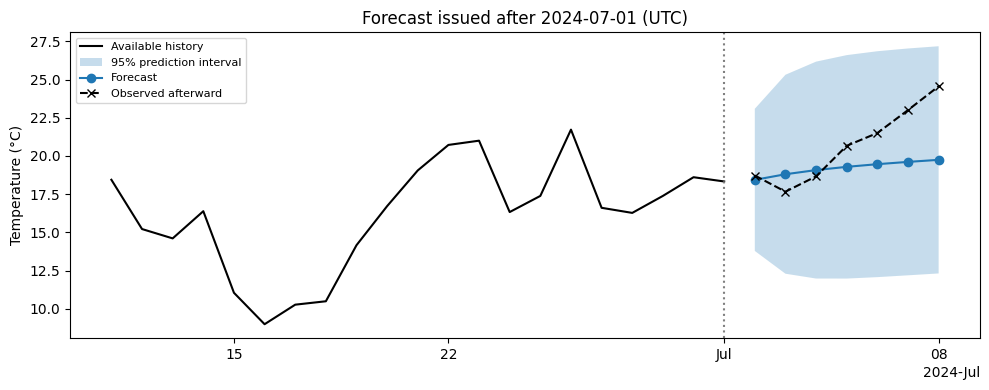
\includegraphics[width=\linewidth]{assets/demo_forecast.png}
\column{.30\textwidth}
\small
\textbf{Notebook, section 6}\par\medskip
Choose \texttt{ORIGIN}.\par\medskip
Filter available history with fixed parameters.\par\medskip
Check against the saved forecast and interval.
\end{columns}
\medskip
\small Demonstration origin: July 1, 2024. Observed future values appear only after forecasting.
\note{7:35--9:20, including 45 seconds of explanation and a 60-second notebook demo. Open section 6 with RUN_PIPELINE=False and ORIGIN=2024-07-01. Run the forecast and plot cells. Explain that observations after the origin do not enter the forecast. Use saved outputs if live execution is unavailable. Source: temperature_forecasting_demo.ipynb.}
\end{frame}

\section{Conclusions}
\begin{frame}{Conclusions and future research}
\textbf{Main findings}\par\medskip
\begin{itemize}
\item Residual dependence improves one-day predictions.
\item Annual seasonality accounts for most seven-day performance.
\item Winter undercoverage limits uncertainty interpretation.
\end{itemize}
\bigskip
\textbf{Next steps}\par\medskip
Additional stations and future test years; flexible variance models and
innovation distributions; meteorological predictors and realistic data-release timing.
\vfill
\scriptsize\url{https://github.com/lamanmirzayeva/Weather-Forecasting}
\note{9:20--10:00. Summarize the horizon dependence and uncertainty limitations. New methods require renewed chronological validation, rather than tuning to the completed 2024 test. Results concern one station and one test year.}
\end{frame}
\end{document}
